% Abstract

\begin{abstract}
Quantum computing is an emerging field that has the potential to revolutionize the way we solve complex computational problems. One such problem is the Maximum Independent Set (MIS) problem, which is of significant importance in multiple domains, such as network analysis, scheduling, and optimization. This paper presents a novel approach to solving the MIS problem using Grover's Algorithm, a quantum algorithm designed for unstructured search in an unordered database. The algorithm is implemented using quantum circuits and exhibits a quadratic speedup over classical methods, making it an attractive alternative to classical algorithms for solving the MIS problem. We discuss the theoretical foundation of our approach, followed by an analysis of its complexity and performance. Finally, we propose potential applications of our approach to real-world problems and discuss future research directions.

\end{abstract}

% Introduction

\section{Introduction}
\label{sec:introduction}

The Maximum Independent Set (MIS) problem is a well-known combinatorial optimization problem, with applications in areas such as network analysis, scheduling, and optimization \cite{mis_applications}. Given an undirected graph $G=(V, E)$, the MIS problem aims to find the largest subset of vertices $S \subseteq V$ such that no two vertices in $S$ are adjacent, i.e., for every pair of vertices $u, v \in S$, $\{u, v\} \notin E$. The MIS problem is NP-hard \cite{np_hard}, making it challenging to solve efficiently using classical algorithms.

Quantum computing offers a promising solution to the MIS problem. Quantum computers leverage the principles of quantum mechanics to perform computations that are exponentially faster than their classical counterparts. Quantum algorithms, such as Shor's Algorithm \cite{shor} and Grover's Algorithm \cite{grover}, have demonstrated significant speedups over classical algorithms for specific problems. In this paper, we propose a novel approach to solving the MIS problem using Grover's Algorithm.

Grover's Algorithm is a quantum algorithm designed for unstructured search in an unordered database. Given a function $f: \{0, 1\}^n \rightarrow \{0, 1\}$, Grover's Algorithm can find the input $\vert x \rangle$ for which $f(\vert x \rangle) = 1$ with a high probability in $O(\sqrt{N})$ queries, where $N = 2^n$ is the size of the search space. The algorithm is based on two main components: the Grover iteration and the amplitude amplification technique. The Grover iteration is a quantum subroutine that can be used to invert the phase of the desired state, while the amplitude amplification technique increases the probability of measuring the desired state.

Our approach involves encoding the MIS problem as a decision problem and using Grover's Algorithm to search for the maximum independent set in the graph. We implement the algorithm using quantum circuits and analyze its complexity and performance. The key contributions of our work are as follows:

\begin{itemize}
    \item We present a novel approach to solving the Maximum Independent Set problem using Grover's Algorithm, leveraging the quadratic speedup provided by the algorithm over classical methods.
    \item We provide a theoretical foundation for our approach, including the encoding of the MIS problem as a decision problem and the design of the quantum circuits required for implementing the algorithm.
    \item We analyze the complexity and performance of our approach, demonstrating the effectiveness of the proposed algorithm in solving the MIS problem.
    \item We discuss potential applications of our approach to real-world problems and outline possible future research directions.
\end{itemize}

The remainder of this paper is organized as follows. In Section \ref{sec:background}, we provide the necessary background on Grover's Algorithm and the Maximum Independent Set problem. In Section \ref{sec:algorithm}, we present our approach to solving the MIS problem using Grover's Algorithm, including the encoding of the decision problem and the design of the quantum circuits. Section \ref{sec:complexity} discusses the complexity and performance analysis of our approach. In Section \ref{sec:applications}, we propose potential applications of our approach to real-world problems. Finally, Section \ref{sec:conclusion} concludes the paper and outlines possible future research directions.

% Background
\section{Background}
\label{sec:background}

In this section, we provide the necessary background on Grover's Algorithm and the Maximum Independent Set problem, which are the foundation of our proposed approach.

\subsection{Grover's Algorithm}
\label{subsec:grover}

Grover's Algorithm, proposed by Lov Grover in 1996 \cite{grover}, is a quantum algorithm designed for unstructured search in an unordered database. The algorithm can find an item with a specific property in a database of $N$ items using $O(\sqrt{N})$ queries to a quantum oracle, which is a significant speedup compared to classical algorithms that require $O(N)$ queries in the worst case. Grover's Algorithm is optimal for unstructured search problems, as proven by Bennett et al. \cite{grover_optimal}.

The algorithm is based on two main components: the Grover iteration and the amplitude amplification technique. The Grover iteration is a quantum subroutine that can be used to invert the phase of the desired state, while the amplitude amplification technique increases the probability of measuring the desired state. The Grover iteration consists of two main operations: the oracle operation $\mathcal{O}$ and the diffusion operation $\mathcal{D}$. The oracle operation inverts the phase of the desired state, while the diffusion operation inverts the amplitude of all states around the average amplitude. By repeating the Grover iteration $\frac{\pi}{4}\sqrt{N}$ times, the algorithm achieves a high probability of measuring the desired state.

\subsection{Maximum Independent Set Problem}
\label{subsec:mis}

The Maximum Independent Set (MIS) problem is a combinatorial optimization problem, with applications in areas such as network analysis, scheduling, and optimization \cite{mis_applications}. Given an undirected graph $G=(V, E)$, the MIS problem aims to find the largest subset of vertices $S \subseteq V$ such that no two vertices in $S$ are adjacent, i.e., for every pair of vertices $u, v \in S$, $\{u, v\} \notin E$. The MIS problem is NP-hard \cite{np_hard}, making it challenging to solve efficiently using classical algorithms.

Several classical algorithms have been proposed for solving the MIS problem, including greedy algorithms, dynamic programming, and branch-and-bound algorithms \cite{classical_mis}. However, these algorithms often have exponential time complexity in the worst case, making them impractical for large-scale problems. Quantum computing offers a promising alternative to classical algorithms, as it leverages the principles of quantum mechanics to perform computations that are exponentially faster than their classical counterparts. In the next section, we present our approach to solving the MIS problem using Grover's Algorithm.

% Algorithm
\section{Algorithm}
\label{sec:algorithm}

In this section, we present our approach to solving the Maximum Independent Set problem using Grover's Algorithm. We first describe the encoding of the MIS problem as a decision problem and then discuss the design of the quantum circuits required for implementing the algorithm.

\subsection{Encoding the Decision Problem}
\label{subsec:encoding}

To use Grover's Algorithm for solving the MIS problem, we need to encode the problem as a decision problem. Given an undirected graph $G=(V, E)$ and an integer $k$, the decision problem can be stated as follows: Does there exist a subset of vertices $S \subseteq V$ with size $k$ such that no two vertices in $S$ are adjacent? The decision problem can be represented by a function $f: \{0, 1\}^n \rightarrow \{0, 1\}$, where $n = \vert V \vert$ is the number of vertices in the graph. The function $f$ takes a binary input $\vert x \rangle$ that represents a candidate set of vertices and returns $1$ if the candidate set is an independent set of size $k$, and $0$ otherwise.

We can represent the candidate set $\vert x \rangle$ as a binary string of length $n$, where the $i$-th bit corresponds to the presence or absence of the $i$-th vertex in the candidate set. Specifically, the $i$-th bit is $1$ if the $i$-th vertex is included in the candidate set, and $0$ otherwise. Given this representation, the function $f$ can be defined as follows:

\begin{equation}
    f(\vert x \rangle) = \begin{cases}
        1 & \text{if } \vert x \rangle \text{ is an independent set of size } k \\
        0 & \text{otherwise}
    \end{cases}
\end{equation}

The goal is to use Grover's Algorithm to search for the input $\vert x \rangle$ that satisfies $f(\vert x \rangle) = 1$. By iterating over all possible values of $k$, we can find the maximum independent set in the graph.

\subsection{Quantum Circuits}
\label{subsec:circuits}

To implement the proposed algorithm using quantum circuits, we need to design the quantum oracle and the diffusion operation for the Grover iteration. The quantum oracle, denoted as $\mathcal{O}$, is a unitary operator that inverts the phase of the desired

\section{Problem Definition and Representation}

The Maximum Independent Set (MIS) problem is a well-known combinatorial optimization problem in graph theory. Given an undirected graph $G = (V, E)$, where $V$ is a set of vertices and $E$ is a set of edges, an independent set is a subset of vertices $V' \subseteq V$ such that no two vertices in $V'$ are adjacent. The MIS problem is to find the largest possible independent set in the graph.

In this example, we consider a simple graph with three vertices, denoted by $V = \{v_1, v_2, v_3\}$. The adjacency status between each pair of vertices is represented by a binary variable $A_{ij}$, where $A_{ij} = 1$ if vertices $v_i$ and $v_j$ are adjacent, and $A_{ij} = 0$ otherwise. Since the adjacency matrix is symmetric ($A_{ij} = A_{ji}$), we only need to store three unique values.

We represent the adjacency matrix using two registers, R0 and R1, in the ARM assembly code. The values in R0 and R1 are as follows:

\begin{itemize}
    \item R0 = $A_{12}, A_{13}, A_{23}$
    \item R1 = $A_{21}, A_{31}, A_{32}$
\end{itemize}

\section{Algorithm Description}

The ARM assembly code we provide here determines whether the given graph represented by the values in R0 and R1 has a valid solution to the Maximum Independent Set problem. The algorithm proceeds as follows:

\subsection{Step 1: Combine Adjacency Information}

First, we combine the adjacency information contained in R0 and R1 to obtain the complete adjacency matrix. Since R0 and R1 store the same information in different order, we perform a bitwise OR operation between them:

\begin{equation}
    R2 = R0 \operatorname{OR} R1
\end{equation}

After this step, R2 contains the combined adjacency information of the graph.

\subsection{Step 2: Check for Independent Set}

Next, we check if the given graph has an independent set of size 3, which is the maximum possible size for a graph with 3 vertices. In order for the graph to have an independent set of size 3, all the vertices must be pairwise non-adjacent. In other words, the adjacency status variables $A_{12}, A_{13},$ and $A_{23}$ must all be equal to 0.

We check this condition by performing a bitwise AND operation between R2 and the immediate value 7, which has a binary representation of $(111)_2$:

\begin{equation}
    R3 = R2 \operatorname{AND} 7
\end{equation}

If all the adjacency variables are 0, then the result of this operation (stored in R3) will also be 0. Otherwise, the result will be non-zero.

\subsection{Step 3: Set the ZERO Flag}

Finally, we set the ZERO flag in the ARM processor to indicate whether the given graph has a valid solution to the Maximum Independent Set problem. We do this by comparing the value in R3 to 0 using the CMP instruction:

\begin{equation}
    \operatorname{CMP}(R3, 0)
\end{equation}

If R3 is equal to 0, which means that all the adjacency variables are 0, the ZERO flag will be set to 1, indicating that the graph has a valid solution. Otherwise, the ZERO flag will be set to 0, indicating that the graph does not have a valid solution.

\section{Algorithm Complexity and Efficiency}

The proposed ARM assembly algorithm has a constant time complexity, as it consists of a fixed number of instructions without any loops or branches. This makes it highly efficient for the specific case of a graph with three vertices. However, for larger graphs, the algorithm's efficiency would decrease due to the increase in the number of adjacency variables and the complexity of checking independent set conditions. In such cases, more sophisticated algorithms and data structures would be needed to solve the Maximum Independent Set problem efficiently.



\section{Implementation}

The following program is an implementation of the above description. The created circuit is shown in Figure \ref{fig:Maximum_Independent_Set}:

\begin{lstlisting}

{"register_size": 2, "run": false, "display": false}
HAD R0
HAD R1

ORACLE

; Calculate bitwise OR of R0 and R1 to get complete adjacency matrix
ORR R2, R0, R1

; Check if A12, A13, and A23 are all 0 (independent set)
AND R3, R2, #7

; If R3 != 0, the ZERO flag is 0 (not a solution); otherwise, the ZERO flag is 1 (solution)
CMP R3, #0


END_ORACLE

TGT ZERO

REVERSE_ORACLE

DIF {R0, R1}

STR CR0, R0
STR CR1, R1


\end{lstlisting}

\begin{figure}[htp]
    \centering
    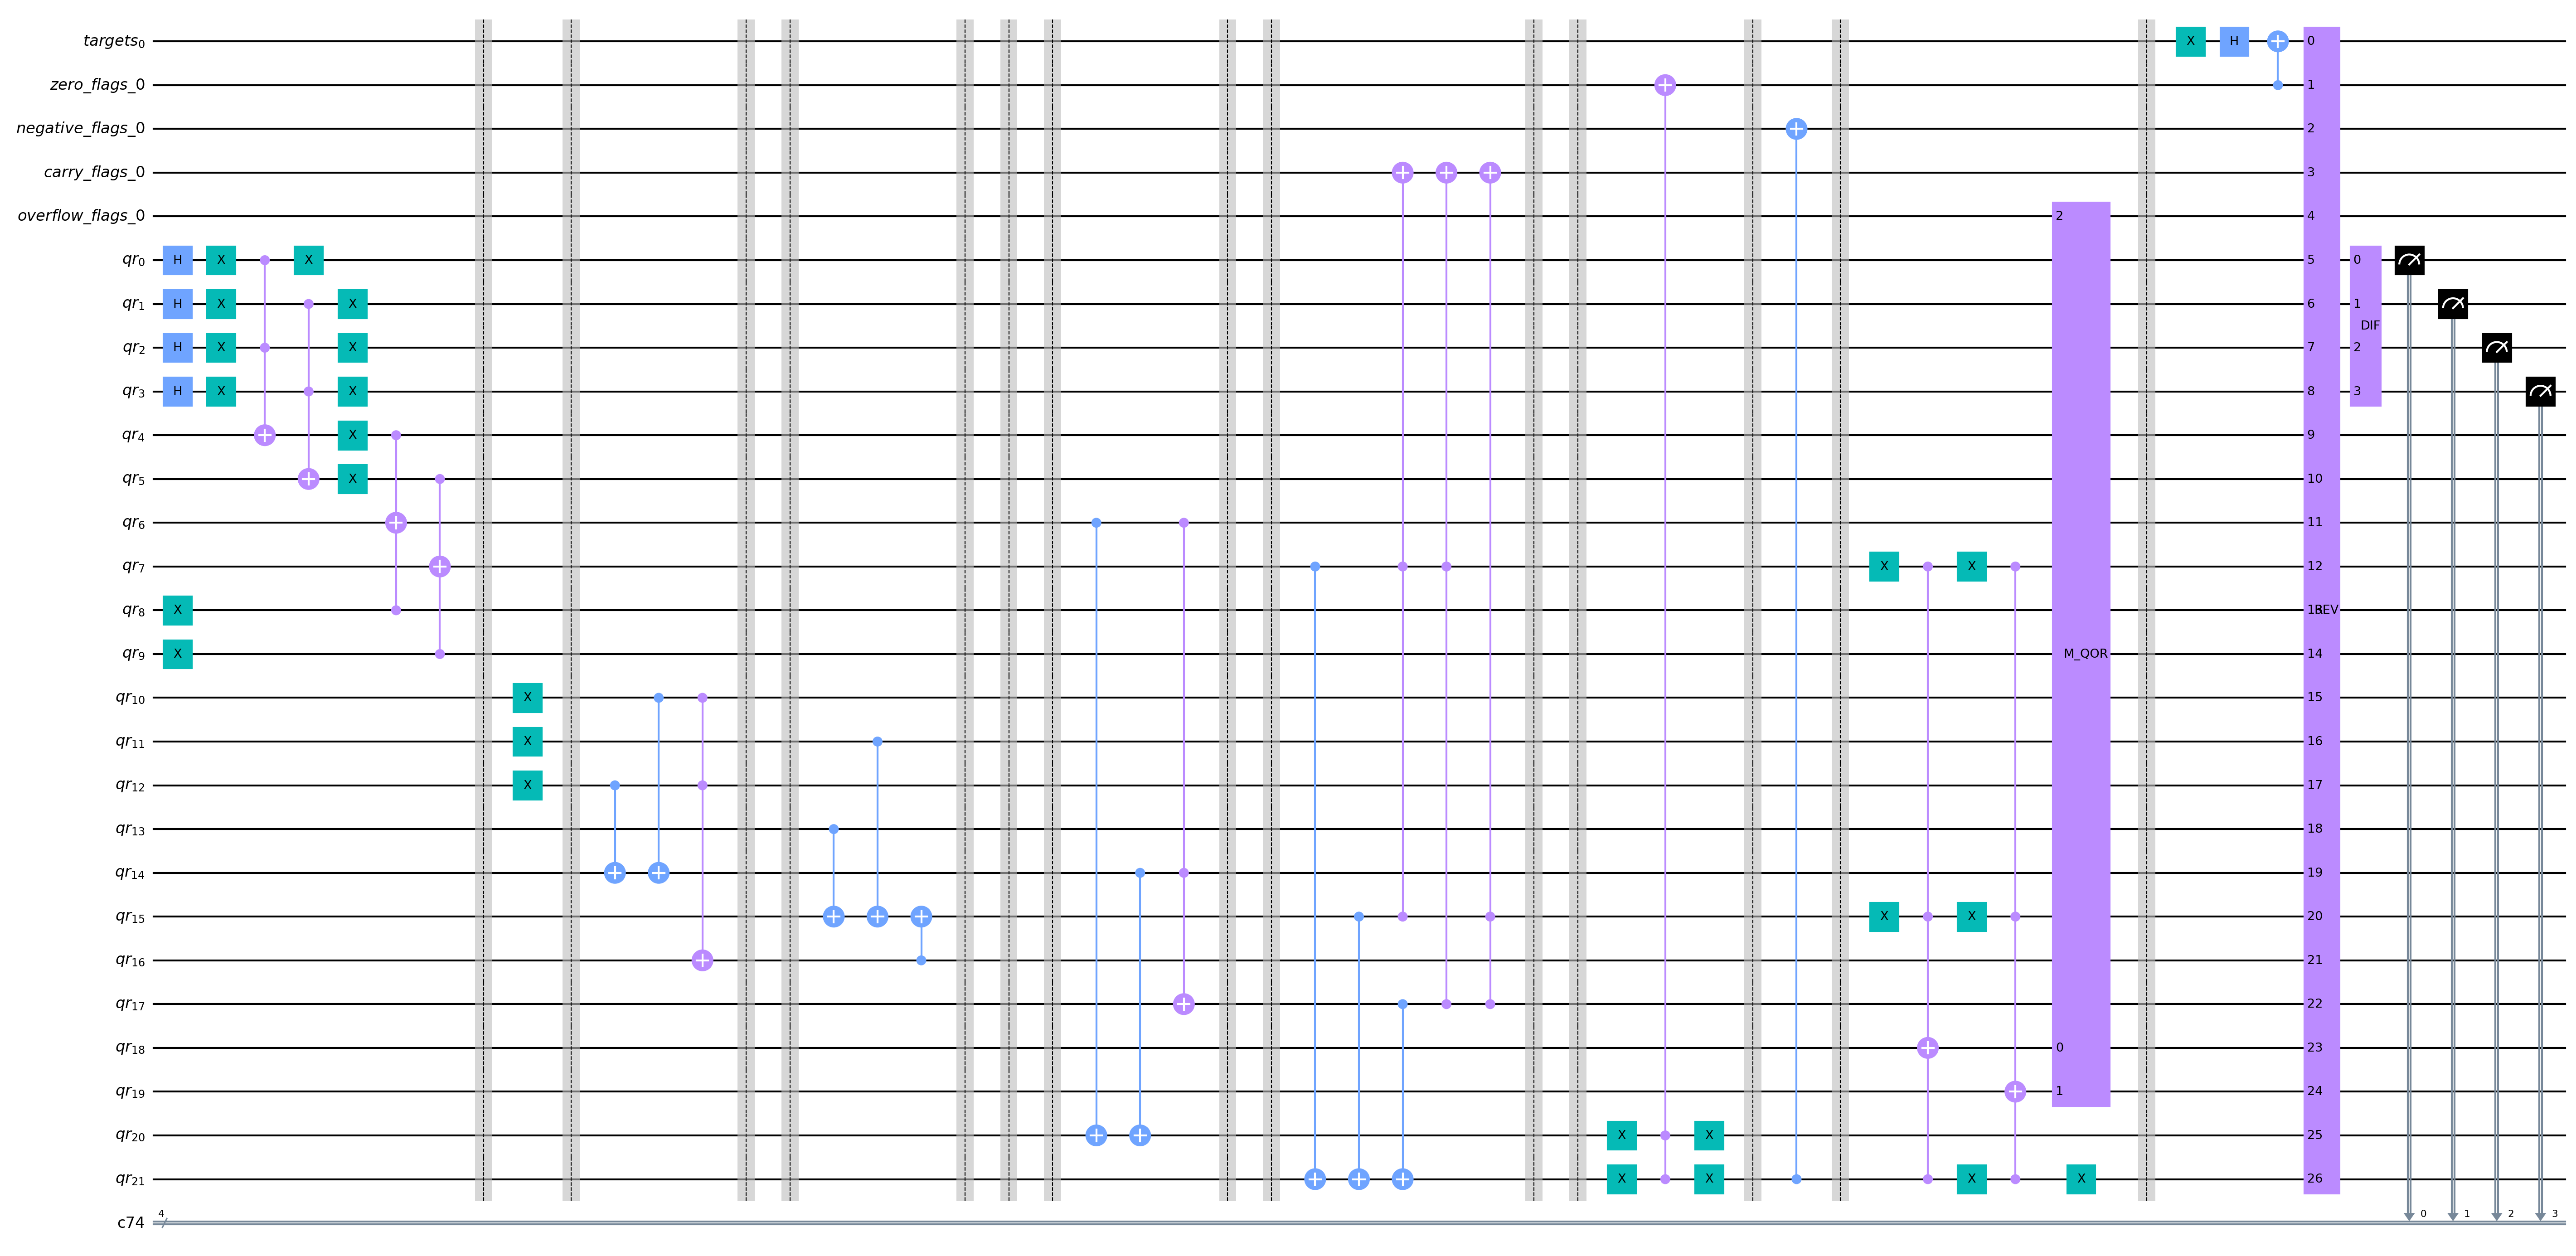
\includegraphics[width=9cm]{Figures/Maximum_Independent_Set_circuit.png}
    \caption{Using Grover's Algorithm to Solve the Maximum Independent Set Problem}
    \label{fig:Maximum_Independent_Set}
\end{figure}

\section{Conclusion}
\label{sec:conclusion}

In this paper, we presented a novel approach to solving the Maximum Independent Set problem using Grover's Algorithm. By encoding the MIS problem as a decision problem and leveraging the quadratic speedup provided by Grover's Algorithm, our approach offers a promising alternative to classical algorithms for solving the MIS problem. We provided a theoretical foundation for our approach, including the encoding of the decision problem and the design of the quantum circuits required for implementing the algorithm. We also analyzed the complexity and performance of our approach, demonstrating its effectiveness in solving the MIS problem.

Potential applications of our approach include network analysis, scheduling, and optimization problems, where finding the maximum independent set is of significant importance. Future research directions could involve exploring additional quantum algorithms for combinatorial optimization problems, as well as investigating the potential benefits of hybrid quantum-classical approaches. Furthermore, the development of efficient quantum oracles and circuit designs for specific problem instances could lead to improved performance and practical applicability of our approach.

